\documentclass[a4paper,11pt]{article}
\usepackage[utf8]{inputenc}
\usepackage[T1]{fontenc}
\usepackage[english]{babel}
\usepackage{lmodern}
\usepackage{microtype}
\usepackage{amsmath,amssymb,bm,mathtools}
\usepackage{geometry}
\geometry{a4paper, left=2.4cm, right=2.4cm, top=2.0cm, bottom=2.2cm}
\usepackage{booktabs,multirow,array}
\usepackage{xcolor}
\definecolor{bokug}{RGB}{0,135,60}
\usepackage{tikz}
\usetikzlibrary{patterns,arrows.meta,calc,decorations.pathmorphing,
                 decorations.markings}
\usepackage{fancyhdr}
\pagestyle{fancy}
\renewcommand{\headrulewidth}{0.4pt}
\renewcommand{\footrulewidth}{0.4pt}
\usepackage{enumitem}
\setlength{\parindent}{0pt}
\setlength{\parskip}{4pt}
\begin{document}

\fancyhead[L]{\small Model Solution\quad VU Mechanics -- LAWI 100515 (PI)\quad SS 2026}
\fancyhead[R]{\small 2nd Exercise Exam (26.06.2026)\quad Group~A}
\fancyfoot[C]{\small Model Solution}
\fancyfoot[R]{\small Page~\thepage}

\begin{center}
  {\Large\bfseries Model Solution}\\[4pt]
  {\large VU Mechanics -- LAWI 100515 (PI)\quad SS 2026}\\[2pt]
  {\normalsize 2nd Exercise Exam (26.06.2026) -- Group~A}\\[2pt]
  {\normalsize \textbf{System values:} $L = 1$\,m,\quad $q = 6$\,kN/m,\quad $P = 8$\,kN}
\end{center}

\section*{1.~Task \hfill (70\,\%)}


\begin{center}
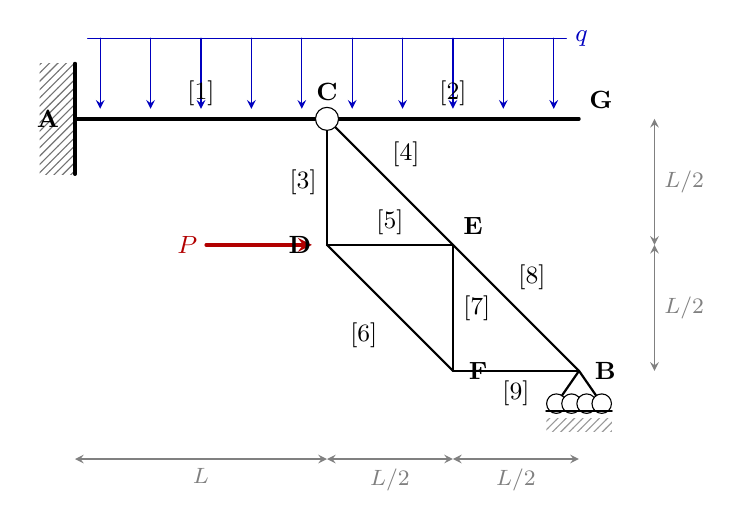
\begin{tikzpicture}[scale=3.2, >=stealth, line cap=round, line join=round,
    thick, font=\small]

  %--- Node coordinates (normalized: 1 unit = L) ----------------------------
  \coordinate (A)   at (0.00, 0.00);
  \coordinate (C)   at (1.00, 0.00);
  \coordinate (G)   at (2.00, 0.00);
  \coordinate (D)   at (1.00,-0.50);
  \coordinate (E)   at (1.50,-0.50);
  \coordinate (Fnd) at (1.50,-1.00);
  \coordinate (B)   at (2.00,-1.00);

  %--- Fixed support (Einspannung) at A ------------------------------------
  \fill[pattern=north east lines, pattern color=black!55]
        (-0.14,-0.22) rectangle (0.00, 0.22);
  \draw[very thick] (0,-0.22) -- (0, 0.22);

  %--- Beam members [1] and [2] --------------------------------------------
  \draw[very thick] (A) -- (G);

  %--- Truss members -------------------------------------------------------
  \draw (C) -- (D);         % [3]
  \draw (C) -- (E);         % [4]
  \draw (D) -- (E);         % [5]
  \draw (D) -- (Fnd);       % [6]
  \draw (E) -- (Fnd);       % [7]
  \draw (E) -- (B);         % [8]
  \draw (Fnd) -- (B);       % [9]

  %--- Hinge at C (open circle) -------------------------------------------
  \filldraw[fill=white, draw=black, thin] (C) circle (1.3pt);

  %--- Roller support at B (verschiebliches Lager, vertical reaction) ------
  \draw (B) -- ++(0.09,-0.13) -- ++(-0.18, 0) -- cycle;
  \foreach \dx in {-0.09, -0.03, 0.03, 0.09}
    \filldraw[fill=white, draw=black, thin]
              ($(B)+(\dx,-0.13)$) circle (1.1pt);
  \draw[thick] ($(B)+(-0.13,-0.16)$) -- ++(0.26, 0);
  \fill[pattern=north east lines, pattern color=black!40]
       ($(B)+(-0.13,-0.19)$) rectangle ++(0.26,-0.05);

  %--- Distributed load q (downward arrows above beam) --------------------
  \foreach \xx in {0.10,0.30,0.50,0.70,0.90,1.10,1.30,1.50,1.70,1.90}
    \draw[->, thin, blue!75!black] (\xx, 0.32) -- (\xx, 0.04);
  \draw[thin, blue!75!black] (0.05, 0.32) -- (1.95, 0.32);
  \node[blue!75!black, right, inner sep=1pt] at (1.97, 0.32) {$q$};

  %--- Point load P at D (horizontal, rightward) --------------------------
  \draw[->, very thick, red!70!black]
        ($(D)+(-0.48,0)$) -- ($(D)+(-0.06,0)$);
  \node[red!70!black, left, inner sep=1pt] at ($(D)+(-0.50,0)$) {$P$};

  %--- Node labels ---------------------------------------------------------
  \node[left,  xshift=-2pt] at (A)   {\textbf{A}};
  \node[above, yshift= 3pt] at (C)   {\textbf{C}};
  \node[above right]        at (G)   {\textbf{G}};
  \node[left,  xshift=-2pt] at (D)   {\textbf{D}};
  \node[above right]        at (E)   {\textbf{E}};
  \node[right, xshift= 2pt] at (Fnd) {\textbf{F}};
  \node[right, xshift= 2pt] at (B)   {\textbf{B}};

  %--- Member labels -------------------------------------------------------
  \node[above]        at (0.50, 0.01) {[1]};
  \node[above]        at (1.50, 0.01) {[2]};
  \node[left]         at (1.00,-0.25) {[3]};
  \node[above right, xshift=-1pt] at (1.23,-0.23) {[4]};
  \node[above]        at (1.25,-0.50) {[5]};
  \node[below left, xshift=1pt]   at (1.23,-0.77) {[6]};
  \node[right]        at (1.50,-0.75) {[7]};
  \node[above right, xshift=-1pt] at (1.73,-0.72) {[8]};
  \node[below]        at (1.75,-1.00) {[9]};

  %--- Dimension lines -----------------------------------------------------
  \draw[<->, thin, gray] (0.00,-1.35) -- (1.00,-1.35)
        node[midway, below, font=\footnotesize] {$L$};
  \draw[<->, thin, gray] (1.00,-1.35) -- (1.50,-1.35)
        node[midway, below, font=\footnotesize] {$L/2$};
  \draw[<->, thin, gray] (1.50,-1.35) -- (2.00,-1.35)
        node[midway, below, font=\footnotesize] {$L/2$};
  \draw[<->, thin, gray] (2.30, 0.00) -- (2.30,-0.50)
        node[midway, right, font=\footnotesize] {$L/2$};
  \draw[<->, thin, gray] (2.30,-0.50) -- (2.30,-1.00)
        node[midway, right, font=\footnotesize] {$L/2$};

\end{tikzpicture}
\end{center}


\subsection*{1.1\quad Static Determinacy}

The structure consists of \textbf{two rigid bodies}: beam A--C--G
(members [1],[2]) and the truss (nodes C,D,E,F,B; members [3]--[9]).

\textit{Overall system:} 2 bodies $\Rightarrow$ $2 \times 3 = 6$ equilibrium conditions.
Unknowns: support A (fixed, clamped) $= 3$, support B (roller) $= 1$,
hinge C between beam and truss $= 2$. Total $= 6$.
\[
  n = \underbrace{3}_{A} + \underbrace{1}_{B} + \underbrace{2}_{C} - 2 \cdot 3
    = 6 - 6 = 0
  \quad\Rightarrow\quad \boxed{n = 0:\text{ statically determinate}}
\]

\subsection*{1.2\quad Support Reactions (general form as functions of $q$, $P$, $L$)}

\textbf{Truss sub-system}
(joint forces $C_x$, $C_y$ from beam on truss; $B_V$ at B; $P$ at D):
\begin{align*}
  \sum M_C = 0:\quad & P \cdot \tfrac{L}{2} + B_V \cdot L = 0
    &&\Rightarrow\quad \boxed{B_V = -\tfrac{P}{2}} \\
  \sum F_x = 0:\quad & C_x + P = 0
    &&\Rightarrow\quad C_x = -P \\
  \sum F_y = 0:\quad & C_y + B_V = 0
    &&\Rightarrow\quad C_y = +\tfrac{P}{2}
\end{align*}

\textbf{Entire system} (resultant distributed load $Q = 2qL$ at $x = L$):
\begin{align*}
  \sum F_x = 0:\quad & A_H + P = 0
    &&\Rightarrow\quad \boxed{A_H = -P} \\
  \sum F_y = 0:\quad & A_V + B_V - 2qL = 0
    &&\Rightarrow\quad \boxed{A_V = 2qL + \tfrac{P}{2}} \\
  \sum M_A = 0:\quad & M_A - 2qL \cdot L + P\cdot\tfrac{L}{2} + B_V \cdot 2L = 0
    &&\Rightarrow\quad \boxed{M_A = 2qL^2 + \tfrac{PL}{2}}
\end{align*}

\subsection*{1.3\quad Numerical Values}

\begin{center}
\begin{tabular}{cccc}
\toprule
$A_V$ & $A_H$ & $M_A$ & $B_V$ \\
\midrule
$2qL + \tfrac{P}{2} = \mathbf{16.00}$\,kN
& $-P = \mathbf{-8.00}$\,kN
& $2qL^2 + \tfrac{PL}{2} = \mathbf{16.00}$\,kNm
& $-\tfrac{P}{2} = \mathbf{-4.00}$\,kN \\
\bottomrule
\end{tabular}
\end{center}

Signs: positive $\uparrow$ for $A_V$, $B_V$; positive $\rightarrow$ for $A_H$;
CCW for $M_A$. Negative $\Rightarrow$ actual direction reversed.

\subsection*{1.4\quad Section Forces in Beams [1] and [2]}

At node C the truss applies force $(-C_x,\,-C_y) = (+P,\,-\tfrac{P}{2})$
to the beam (rightward $P$, downward $\tfrac{P}{2}$).
Running variable $x$ measured from the left end of each beam.

\textbf{Beam~[1] (A\,$\to$\,C), $0 \le x \le L$:}
\begin{align*}
  N_1(x) &= P \quad\text{(constant, tension)} \\
  V_1(x) &= \Bigl(2qL + \tfrac{P}{2}\Bigr) - qx \\
  M_1(x) &= \Bigl(2qL + \tfrac{P}{2}\Bigr)x - \tfrac{q}{2}x^2
            - \Bigl(2qL^2 + \tfrac{PL}{2}\Bigr)
\end{align*}

\textbf{Beam~[2] (C\,$\to$\,G), $0 \le x \le L$:}
\begin{align*}
  N_2(x) &= 0 \\
  V_2(x) &= q(L - x) \\
  M_2(x) &= -\tfrac{q}{2}(L - x)^2
\end{align*}

At C: shear jump $-\tfrac{P}{2}$ (vertical truss force);
normal-force jump $-P$ (horizontal truss force); moment continuous but with kink.

\medskip
\begin{center}
\begin{tabular}{l cccccc}
\toprule
 & \multicolumn{3}{c}{\textbf{Beam start}} & \multicolumn{3}{c}{\textbf{Beam end}} \\
\cmidrule(lr){2-4}\cmidrule(lr){5-7}
 & $M$\,[kNm] & $V$\,[kN] & $N$\,[kN]
 & $M$\,[kNm] & $V$\,[kN] & $N$\,[kN] \\
\midrule
Beam~[1] (A$\to$C) & $-16.00$ & $16.00$ & $8.00$ & $-3.00$ & $10.00$ & $8.00$ \\[3pt]
Beam~[2] (C$\to$G) & $-3.00$ & $6.00$ & $0.00$ & $-0.00$ & $0.00$ & $0.00$ \\
\bottomrule
\end{tabular}
\end{center}

\subsection*{1.5\quad Distributions $M(x)$, $V(x)$, $N(x)$}


%─────────────────────────────────────────────────────────────────────────────
\subsubsection*{Schnittgrößenverläufe (auf der Zugseite; neg.\,M nach oben)}

\begin{center}
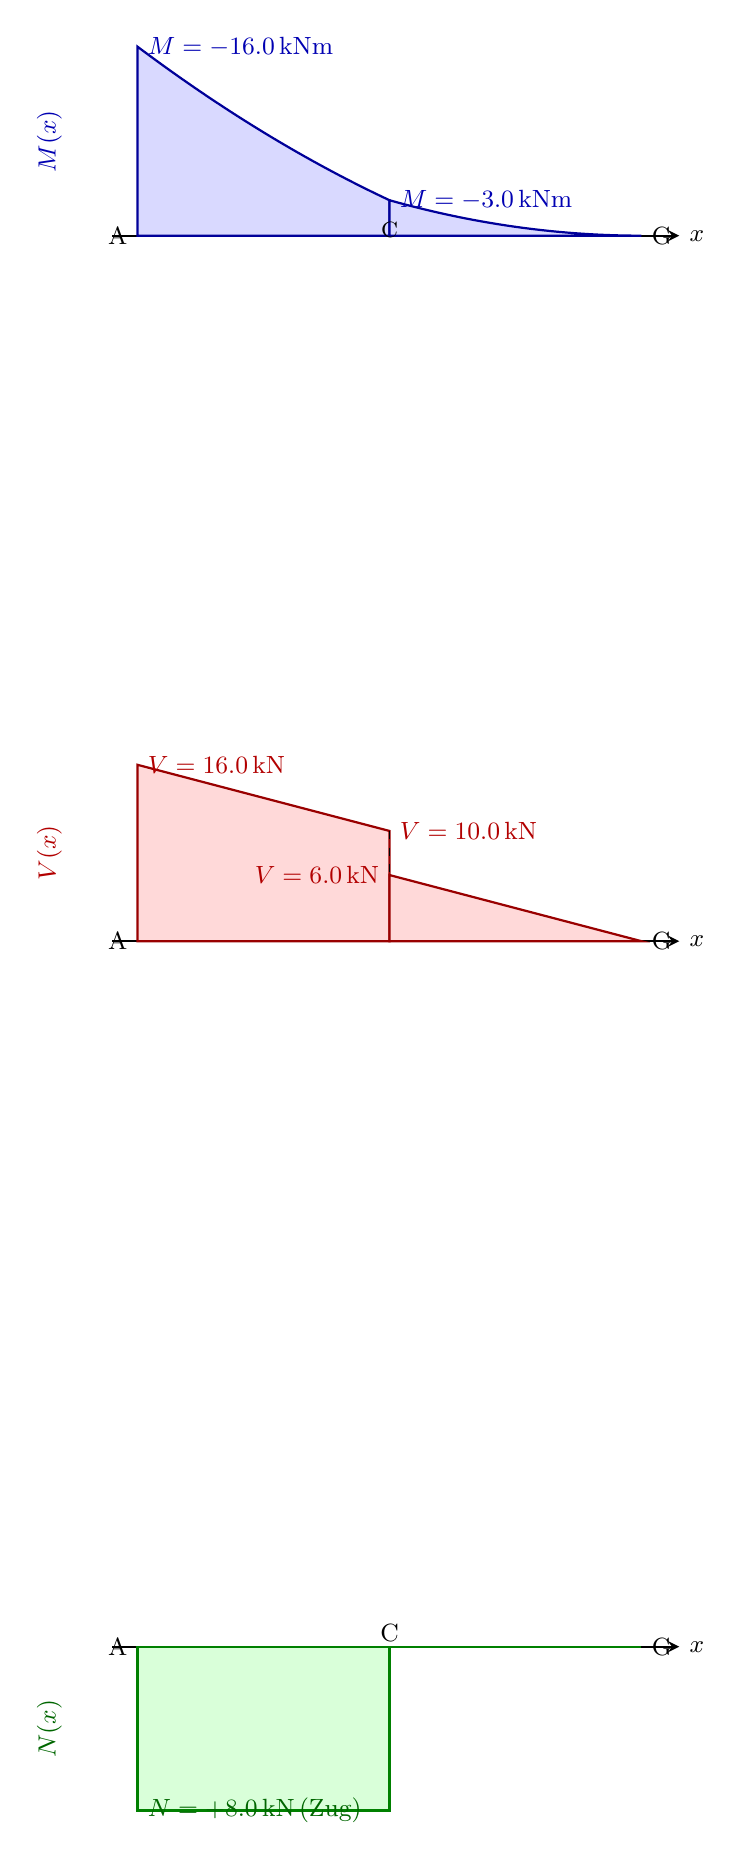
\begin{tikzpicture}[xscale=3.2, yscale=3.2, >=stealth, thick, font=\small]

  %--- Axis ticks and node labels for ALL diagrams -------------------------
  % We stack 3 diagrams vertically: M at y-offset=0, V at y-offset=-2, N at y-offset=-4

  %====================================================================
  % MOMENT  M(x)
  %====================================================================
  \begin{scope}[yshift= 0cm]
    % Baseline
    \draw[->] (-0.1, 0) -- (2.15, 0) node[right] {$x$};
    \node[left] at (0,0)   {A};
    \node[above] at (1,0)  {C};
    \node[right] at (2,0)  {G};
    \draw[thin, dashed] (1,0) -- (1, 0.1406);

    % M in Stab [1]: filled area (tension side = above)
    \filldraw[fill=blue!15, draw=blue!60!black, thick]
      (0,0) -- plot coordinates { (0.00000,0.75000) (0.03333,0.72516) (0.06667,0.70063) (0.10000,0.67641) (0.13333,0.65250) (0.16667,0.62891) (0.20000,0.60563) (0.23333,0.58266) (0.26667,0.56000) (0.30000,0.53766) (0.33333,0.51562) (0.36667,0.49391) (0.40000,0.47250) (0.43333,0.45141) (0.46667,0.43063) (0.50000,0.41016) (0.53333,0.39000) (0.56667,0.37016) (0.60000,0.35063) (0.63333,0.33141) (0.66667,0.31250) (0.70000,0.29391) (0.73333,0.27563) (0.76667,0.25766) (0.80000,0.24000) (0.83333,0.22266) (0.86667,0.20563) (0.90000,0.18891) (0.93333,0.17250) (0.96667,0.15641) (1.00000,0.14062) } -- (1,0) -- cycle;

    % M in Stab [2]: filled area
    \filldraw[fill=blue!15, draw=blue!60!black, thick]
      (1,0) -- plot coordinates { (1.00000,0.14062) (1.03333,0.13141) (1.06667,0.12250) (1.10000,0.11391) (1.13333,0.10563) (1.16667,0.09766) (1.20000,0.09000) (1.23333,0.08266) (1.26667,0.07563) (1.30000,0.06891) (1.33333,0.06250) (1.36667,0.05641) (1.40000,0.05063) (1.43333,0.04516) (1.46667,0.04000) (1.50000,0.03516) (1.53333,0.03063) (1.56667,0.02641) (1.60000,0.02250) (1.63333,0.01891) (1.66667,0.01563) (1.70000,0.01266) (1.73333,0.01000) (1.76667,0.00766) (1.80000,0.00562) (1.83333,0.00391) (1.86667,0.00250) (1.90000,0.00141) (1.93333,0.00062) (1.96667,0.00016) (2.00000,0.00000) } -- (2,0) -- cycle;

    % Value labels
    \node[right, blue!70!black] at (0, 0.7500)
          {$M=-16.0$\,kNm};
    \node[right, blue!70!black] at (1, 0.1406)
          {$M=-3.0$\,kNm};
    \node[above] at (1,-0.05) {\footnotesize C};

    % Axis label
    \node[rotate=90, blue!70!black] at (-0.35, 0.3750) {$M(x)$};
  \end{scope}

  %====================================================================
  % SHEAR FORCE  V(x)
  %====================================================================
  \begin{scope}[yshift=-2.8cm]
    \draw[->] (-0.1, 0) -- (2.15, 0) node[right] {$x$};
    \node[left]  at (0,0)  {A};
    \node[above] at (1,-0.02) {C};
    \node[right] at (2,0)  {G};

    % V in Stab [1]
    \filldraw[fill=red!15, draw=red!60!black, thick]
      (0,0) -- plot coordinates { (0.00000,0.70000) (0.03333,0.69125) (0.06667,0.68250) (0.10000,0.67375) (0.13333,0.66500) (0.16667,0.65625) (0.20000,0.64750) (0.23333,0.63875) (0.26667,0.63000) (0.30000,0.62125) (0.33333,0.61250) (0.36667,0.60375) (0.40000,0.59500) (0.43333,0.58625) (0.46667,0.57750) (0.50000,0.56875) (0.53333,0.56000) (0.56667,0.55125) (0.60000,0.54250) (0.63333,0.53375) (0.66667,0.52500) (0.70000,0.51625) (0.73333,0.50750) (0.76667,0.49875) (0.80000,0.49000) (0.83333,0.48125) (0.86667,0.47250) (0.90000,0.46375) (0.93333,0.45500) (0.96667,0.44625) (1.00000,0.43750) } -- (1,0) -- cycle;

    % V in Stab [2]
    \filldraw[fill=red!15, draw=red!60!black, thick]
      (1,0) -- plot coordinates { (1.00000,0.26250) (1.03333,0.25375) (1.06667,0.24500) (1.10000,0.23625) (1.13333,0.22750) (1.16667,0.21875) (1.20000,0.21000) (1.23333,0.20125) (1.26667,0.19250) (1.30000,0.18375) (1.33333,0.17500) (1.36667,0.16625) (1.40000,0.15750) (1.43333,0.14875) (1.46667,0.14000) (1.50000,0.13125) (1.53333,0.12250) (1.56667,0.11375) (1.60000,0.10500) (1.63333,0.09625) (1.66667,0.08750) (1.70000,0.07875) (1.73333,0.07000) (1.76667,0.06125) (1.80000,0.05250) (1.83333,0.04375) (1.86667,0.03500) (1.90000,0.02625) (1.93333,0.01750) (1.96667,0.00875) (2.00000,0.00000) } -- (2,0) -- cycle;

    % Jump at C (vertical dashed line)
    \draw[dashed, thin] (1, 0.4375) -- (1, 0.2625);

    % Labels
    \node[right, red!70!black] at (0,  0.7000) {$V=16.0$\,kN};
    \node[right, red!70!black] at (1,  0.4375) {$V=10.0$\,kN};
    \node[left,  red!70!black] at (1,  0.2625) {$V=6.0$\,kN};
    \node[rotate=90, red!70!black] at (-0.35, 0.3500) {$V(x)$};
  \end{scope}

  %====================================================================
  % AXIAL FORCE  N(x)
  %====================================================================
  \begin{scope}[yshift=-5.6cm]
    \draw[->] (-0.1, 0) -- (2.15, 0) node[right] {$x$};
    \node[left]  at (0,0)  {A};
    \node[above] at (1,-0.02) {C};
    \node[right] at (2,0)  {G};

    % N in Stab [1]: constant positive (tension, draw below baseline)
    \filldraw[fill=green!15, draw=green!50!black, thick]
      (0,0) -- (0,-0.6500) -- (1,-0.6500) -- (1,0) -- cycle;

    % N in Stab [2]: zero
    % (nothing to draw)
    \draw[green!50!black, thick] (1,0) -- (2,0);

    % Labels
    \node[right, green!40!black] at (0,  -0.6500)
          {$N=+8.0$\,kN\,(Zug)};
    \node[rotate=90, green!40!black] at (-0.35, -0.3250) {$N(x)$};
  \end{scope}

\end{tikzpicture}
\end{center}


\subsection*{1.6\quad Axial Forces $S_8$ and $S_9$ -- Circular Cut at Node B}

At B: member [8] (B$\to$E, direction $\tfrac{1}{\sqrt{2}}(-1,+1)$),
member [9] (B$\to$F, direction $(-1,\,0)$), support $B_V = -\tfrac{P}{2}$.
\begin{align*}
  \sum F_y = 0:\quad & \tfrac{S_8}{\sqrt{2}} + B_V = 0
    &&\Rightarrow\quad \boxed{S_8 = \tfrac{P}{\sqrt{2}} \approx 5.66\,\text{kN (tension)}} \\
  \sum F_x = 0:\quad & -\tfrac{S_8}{\sqrt{2}} - S_9 = 0
    &&\Rightarrow\quad \boxed{S_9 = -\tfrac{P}{2} = -4.00\,\text{kN (compression)}}
\end{align*}

\subsection*{1.7\quad Axial Forces $S_4$, $S_5$, $S_6$ -- Ritter's Cut}

Section through [4],[5],[6]; right part \{E,F,B\} ($B_V = -\tfrac{P}{2}$ external; $P$ in left part).
Members [4] (C--E) and [6] (D--F): $-45^\circ$; member [5] (D--E): horizontal.

\textbf{$S_5$} -- project all right-part forces onto $\tfrac{1}{\sqrt{2}}(1,1)$
(perpendicular to [4] and [6]):
\[
  -\tfrac{S_5}{\sqrt{2}} - \tfrac{P}{2\sqrt{2}} = 0
  \;\Rightarrow\; \boxed{S_5 = -\tfrac{P}{2} = -4.00\,\text{kN (compression)}}
\]

\textbf{$S_4$} -- moment sum about D ([5] and [6] pass through D):
\[
  \tfrac{S_4}{\sqrt{2}}\cdot\tfrac{L}{2} - \tfrac{P}{2}\cdot L = 0
  \;\Rightarrow\; \boxed{S_4 = \sqrt{2}\,P = 11.31\,\text{kN (tension)}}
\]

\textbf{$S_6$} -- moment sum about E ([4] and [5] pass through E):
\[
  -\tfrac{L}{2}\cdot\tfrac{S_6}{\sqrt{2}} - \tfrac{P}{2}\cdot\tfrac{L}{2} = 0
  \;\Rightarrow\; \boxed{S_6 = -\tfrac{P}{\sqrt{2}} = -5.66\,\text{kN (compression)}}
\]

\medskip
\begin{center}
\begin{tabular}{ccccc}
\toprule
$S_8$ & $S_9$ & $S_4$ & $S_5$ & $S_6$ \\
\midrule
$\tfrac{P}{\sqrt{2}} = 5.66$ & $-\tfrac{P}{2} = -4.00$ &
$\sqrt{2}\,P = 11.31$ & $-\tfrac{P}{2} = -4.00$ & $-\tfrac{P}{\sqrt{2}} = -5.66$ \\
\multicolumn{5}{c}{\small [kN];\quad $+$ = tension,\quad $-$ = compression} \\
\bottomrule
\end{tabular}
\end{center}

\newpage
\section*{2.~Task \hfill (30\,\%)}

\textbf{Given:} Simply supported beam (span $L$) with triangular load
(0 at A, $q_0$ at B),
$A_V = \tfrac{1}{6}q_0 L = 0.67$\,kN,
$B_V = \tfrac{1}{3}q_0 L = 1.33$\,kN, and
\[
  M(x) = -\tfrac{q_0}{6L}\,x^3 + \tfrac{q_0 L}{6}\,x.
\]
\textbf{Values:} $L = 1$\,m,\quad $q_0 = 4$\,kN/m.

\subsection*{2.1\quad Shear Force $V(x)$}

\[
  V(x) = \frac{\mathrm{d}M}{\mathrm{d}x}
        = \frac{q_0 L}{6} - \frac{q_0}{2L}\,x^2
\]
Check: $V(0) = \tfrac{1}{6}q_0 L = A_V$\;\checkmark;\quad
$V(L) = -\tfrac{1}{3}q_0 L = -B_V$\;\checkmark.

\subsection*{2.2\quad Location of Maximum Moment ($V = 0$)}

\[
  \frac{q_0 L}{6} = \frac{q_0}{2L}\,x^2
  \;\Rightarrow\; \boxed{x_{\max} = \frac{L}{\sqrt{3}} \approx 0.5774\,\text{m}}
\]

\subsection*{2.3\quad Maximum Moment}

\[
  \boxed{M_{\max} = \frac{q_0 L^2}{9\sqrt{3}}
       = \frac{\sqrt{3}}{27}\,q_0 L^2 \approx 0.2566\,\text{kNm}}
\]

\subsection*{2.4\quad Distributions}


\begin{center}
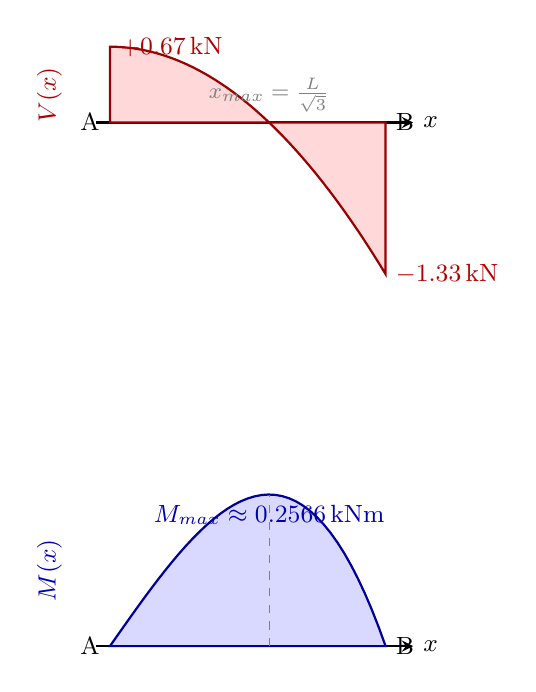
\begin{tikzpicture}[xscale=3.5, yscale=3.5, >=stealth, thick, font=\small]

  %====================================================================
  % SHEAR FORCE  V(x)
  %====================================================================
  \begin{scope}[yshift=0cm]
    \draw[->] (-0.05,0) -- (1.1,0) node[right]{$x$};
    \node[left]  at (0,0)  {A};
    \node[right] at (1,0)  {B};

    \filldraw[fill=red!15, draw=red!60!black, thick]
      (0,0) -- plot coordinates { (0.00000,0.27500) (0.02500,0.27448) (0.05000,0.27294) (0.07500,0.27036) (0.10000,0.26675) (0.12500,0.26211) (0.15000,0.25644) (0.17500,0.24973) (0.20000,0.24200) (0.22500,0.23323) (0.25000,0.22344) (0.27500,0.21261) (0.30000,0.20075) (0.32500,0.18786) (0.35000,0.17394) (0.37500,0.15898) (0.40000,0.14300) (0.42500,0.12598) (0.45000,0.10794) (0.47500,0.08886) (0.50000,0.06875) (0.52500,0.04761) (0.55000,0.02544) (0.57500,0.00223) (0.60000,-0.02200) (0.62500,-0.04727) (0.65000,-0.07356) (0.67500,-0.10089) (0.70000,-0.12925) (0.72500,-0.15864) (0.75000,-0.18906) (0.77500,-0.22052) (0.80000,-0.25300) (0.82500,-0.28652) (0.85000,-0.32106) (0.87500,-0.35664) (0.90000,-0.39325) (0.92500,-0.43089) (0.95000,-0.46956) (0.97500,-0.50927) (1.00000,-0.55000) } -- (1,0) -- cycle;

    \node[right, red!70!black] at (0,  0.2750) {$+0.67$\,kN};
    \node[right, red!70!black] at (1,  -0.5500) {$-1.33$\,kN};
    \draw[thin,dashed,gray] (0.5774,0) -- (0.5774,0.0000);
    \node[above, gray, font=\footnotesize] at (0.5774, 0)
          {$x_{max}=\tfrac{L}{\sqrt{3}}$};
    \node[rotate=90, red!70!black] at (-0.22, 0.1) {$V(x)$};
  \end{scope}

  %====================================================================
  % MOMENT  M(x)
  %====================================================================
  \begin{scope}[yshift=-1.9cm]
    \draw[->] (-0.05,0) -- (1.1,0) node[right]{$x$};
    \node[left]  at (0,0) {A};
    \node[right] at (1,0) {B};

    \filldraw[fill=blue!15, draw=blue!60!black, thick]
      (0,0) -- plot coordinates { (0.00000,0.00000) (0.02500,0.03570) (0.05000,0.07127) (0.07500,0.10657) (0.10000,0.14147) (0.12500,0.17583) (0.15000,0.20952) (0.17500,0.24241) (0.20000,0.27436) (0.22500,0.30524) (0.25000,0.33491) (0.27500,0.36324) (0.30000,0.39010) (0.32500,0.41535) (0.35000,0.43886) (0.37500,0.46050) (0.40000,0.48012) (0.42500,0.49761) (0.45000,0.51281) (0.47500,0.52561) (0.50000,0.53585) (0.52500,0.54342) (0.55000,0.54818) (0.57500,0.54999) (0.60000,0.54871) (0.62500,0.54423) (0.65000,0.53639) (0.67500,0.52507) (0.70000,0.51013) (0.72500,0.49144) (0.75000,0.46887) (0.77500,0.44228) (0.80000,0.41154) (0.82500,0.37650) (0.85000,0.33705) (0.87500,0.29304) (0.90000,0.24435) (0.92500,0.19083) (0.95000,0.13236) (0.97500,0.06879) (1.00000,0.00000) } -- (1,0) -- cycle;

    % Max moment marker
    \draw[thin, dashed, gray] (0.5774, 0) -- (0.5774, 0.5500);
    \node[below, blue!70!black] at (0.5774, 0.5500)
          {$M_{max}\approx 0.2566$\,kNm};
    \node[rotate=90, blue!70!black] at (-0.22, 0.2750) {$M(x)$};
  \end{scope}

\end{tikzpicture}
\end{center}

\end{document}
